% !TEX program = xelatex
\documentclass[10pt,aspectratio=169]{beamer}

\setbeamersize{text margin left=5mm,text margin right=5mm} 

\usepackage{amsthm,amsmath,amssymb,braket,fontspec}
\usepackage[absolute,overlay]{textpos}

\usetheme{metropolis}
\usecolortheme{beaver}
\setbeamercolor{frametitle}{bg=gray,fg=red}
\setsansfont{Fira Sans}
\setbeamertemplate{footline}{}

\usepackage[backend=bibtex,url=false,doi=false,style=authoryear]{biblatex}
\bibliography{aux_model}
\AtBeginBibliography{\scriptsize}

\newcommand{\focus}[1]{\textcolor{lblue}{\textbf{#1}}}
\renewcommand{\thefootnote}{}
\renewcommand*\footnoterule{}

\definecolor{gray}{HTML}{E0E0E0}
\definecolor{lblue}{HTML}{4169E1}
\definecolor{red}{HTML}{CC0000}
\setbeamertemplate{bibliography item}[triangle]

\AtBeginSection[]{
\begin{frame}[noframenumbering]
  \vfill
  \centering
  \begin{beamercolorbox}[sep=20pt,rounded=true,center]{frametitle}
    \usebeamerfont{title}\insertsectionhead\par%
  \end{beamercolorbox}
  \vfill
\end{frame}
}
\title{
{Local metal-insulator transition in a generalised Anderson impurity model}
}
\date{\today}
\author{\large Abhirup Mukherjee, Siddhartha Lal}
\institute{Department of Physical Sciences, IISER Kolkata, Mohanpur}
\date{\large\today}

\begin{document}

\begin{frame}[noframenumbering]
\maketitle
\begin{textblock*}{0.7\textwidth}(7.5cm, 5.5cm)
	\centering
	\vspace*{\fill}

	\hspace*{\fill}
	
\includegraphics[width=0.2\textwidth]{figures/epqm_logo_mod.jpeg}
	
\includegraphics[width=0.2\textwidth]{figures/dps_logo.jpeg}
	\hspace*{\fill}

	\vspace*{\fill}
\end{textblock*}
\end{frame}

\section{Why another impurity model?}

\begin{frame}[noframenumbering]{Anderson and Kondo impurity models - No transition!}

\hspace*{-20pt}
\begin{minipage}{0.53\textwidth}
\begin{itemize}
	\item simplest - Anderson and Kondo models\\[20pt]
	\item localisation physics + hybridisation\\[20pt]
	\item screened at low \(T\)\\[20pt]
\end{itemize}
\end{minipage}
\begin{minipage}{0.5\textwidth}
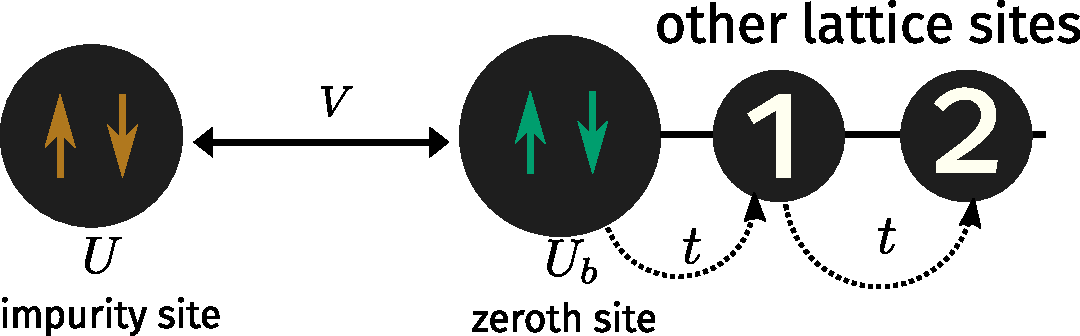
\includegraphics[width=0.99\textwidth]{figures/siam.pdf}
\end{minipage}
\end{frame}

\section{Brief Summary of Results}
\begin{frame}[noframenumbering]{Brief Summary of Results}
\begin{itemize}[<+->]
	\item Competition between Kondo interaction and local attractive interaction causes \focus{impurity phase transition}.\\[20pt]
	\item Transition involves growth of \focus{charge content}, finally leading to local moment.\\[20pt]
	\item \focus{Spectral function} goes through a three-peak structure at the critical point, and develops a gap beyond that.\\[20pt]
	\item Geometric \focus{entanglement} acts as an order parameter for the transition.
\end{itemize}
\end{frame}

\section{Outline}
\begin{frame}[noframenumbering]{Outline}
\begin{itemize}[<alert@+>]
	\item[1.] {The generalised Anderson impurity model}\\[10pt]
	\item[2.] {Short description of the unitary RG method}\\[10pt]
	\item[3.] {RG equations, phase diagram and phase transition}\\[10pt]
	\item[4.] {Effective Hamiltonian and ground state}\\[10pt]
	\item[5.] {Description of phase transition through spectral functions and entanglement}\\[10pt]
	\item[6.] {Some concluding remarks}
\end{itemize}
\end{frame}

\section{The Model}
\label{the-model}
\begin{frame}[noframenumbering]{The Model}
\centering
	{\large\(H = \overbrace{\sum_{k\sigma}\epsilon_k \tau_{k\sigma} + V \sum_{k\sigma}\left(c^\dagger_{d\sigma}c_{k\sigma} + \text{h.c.}\right)  - \frac{1}{2}U \left(\hat n_{d \uparrow} - \hat n_{d \downarrow}\right)^2}^\text{\large p-h symmetric Anderson impurity model} + \underbrace{J \vec{S}_d\cdot\vec{S}_0 - U_b \left(\hat n_{0 \uparrow} - \hat n_{0 \downarrow}\right)^2}_\text{\large additional terms}\)}

\vspace*{\fill}
\hspace*{-25pt}
\begin{minipage}{0.39\textwidth}
\begin{itemize}
	\item \focus{spin-exchange} between impurity and bath
	\item \focus{correlation} on zeroth site of bath
\end{itemize}
\end{minipage}
\begin{minipage}{0.6\textwidth}
\hspace*{15pt}
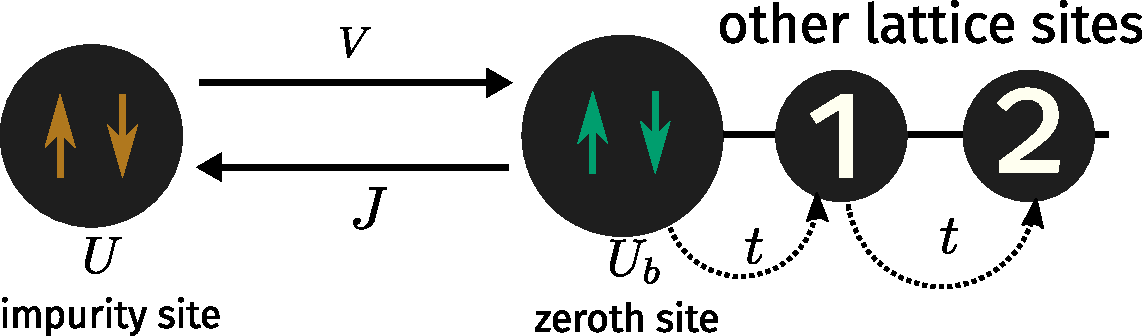
\includegraphics[width=0.95\textwidth]{figures/zeromode_bare.pdf}
\end{minipage}

\footcite{Schrieffer_Wolff,anderson_impurity_1961}

\end{frame}

\section{The Unitary Renormalization Group Method}
\label{method}
\begin{frame}[noframenumbering]{The Unitary RG Method: The General Idea}
\footcite{anirbanurg1,anirbanurg2}

\begin{minipage}{0.8\textwidth}
\begin{itemize}[<+->]
	\item Apply unitary many-body transformations to the Hamiltonian\\[10pt]
	\item Successively decouple high energy states\\[10pt]
	\item Obtain sequence of Hamiltonians and hence scaling equations
\end{itemize}
\end{minipage}
\begin{minipage}{0.15\textwidth}
\begin{figure}
	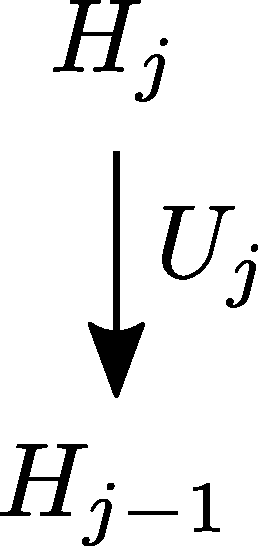
\includegraphics[width=0.7\textwidth]{figures/urg_schematic.pdf}
\end{figure}
\end{minipage}
\end{frame}

\begin{frame}[noframenumbering]{The Unitary RG Method: Select a UV-IR Scheme}
\vspace*{\fill}

\begin{minipage}{0.5\textwidth}
\centering
\focus{UV shell}
\begin{gather*}
	\vec k_N ~~ \left(\text{zeroth RG step}\right)\\
\vdots\\ 
\vec k_j ~ ~ \left(j^\text{th} \text{ RG step}\right) \\
\vdots\\
\vec k_1 ~ ~ \left(\text{Fermi surface}\right)
\end{gather*}
\focus{IR shell}
\end{minipage}
\hspace*{\fill}
\begin{minipage}{0.4\textwidth}
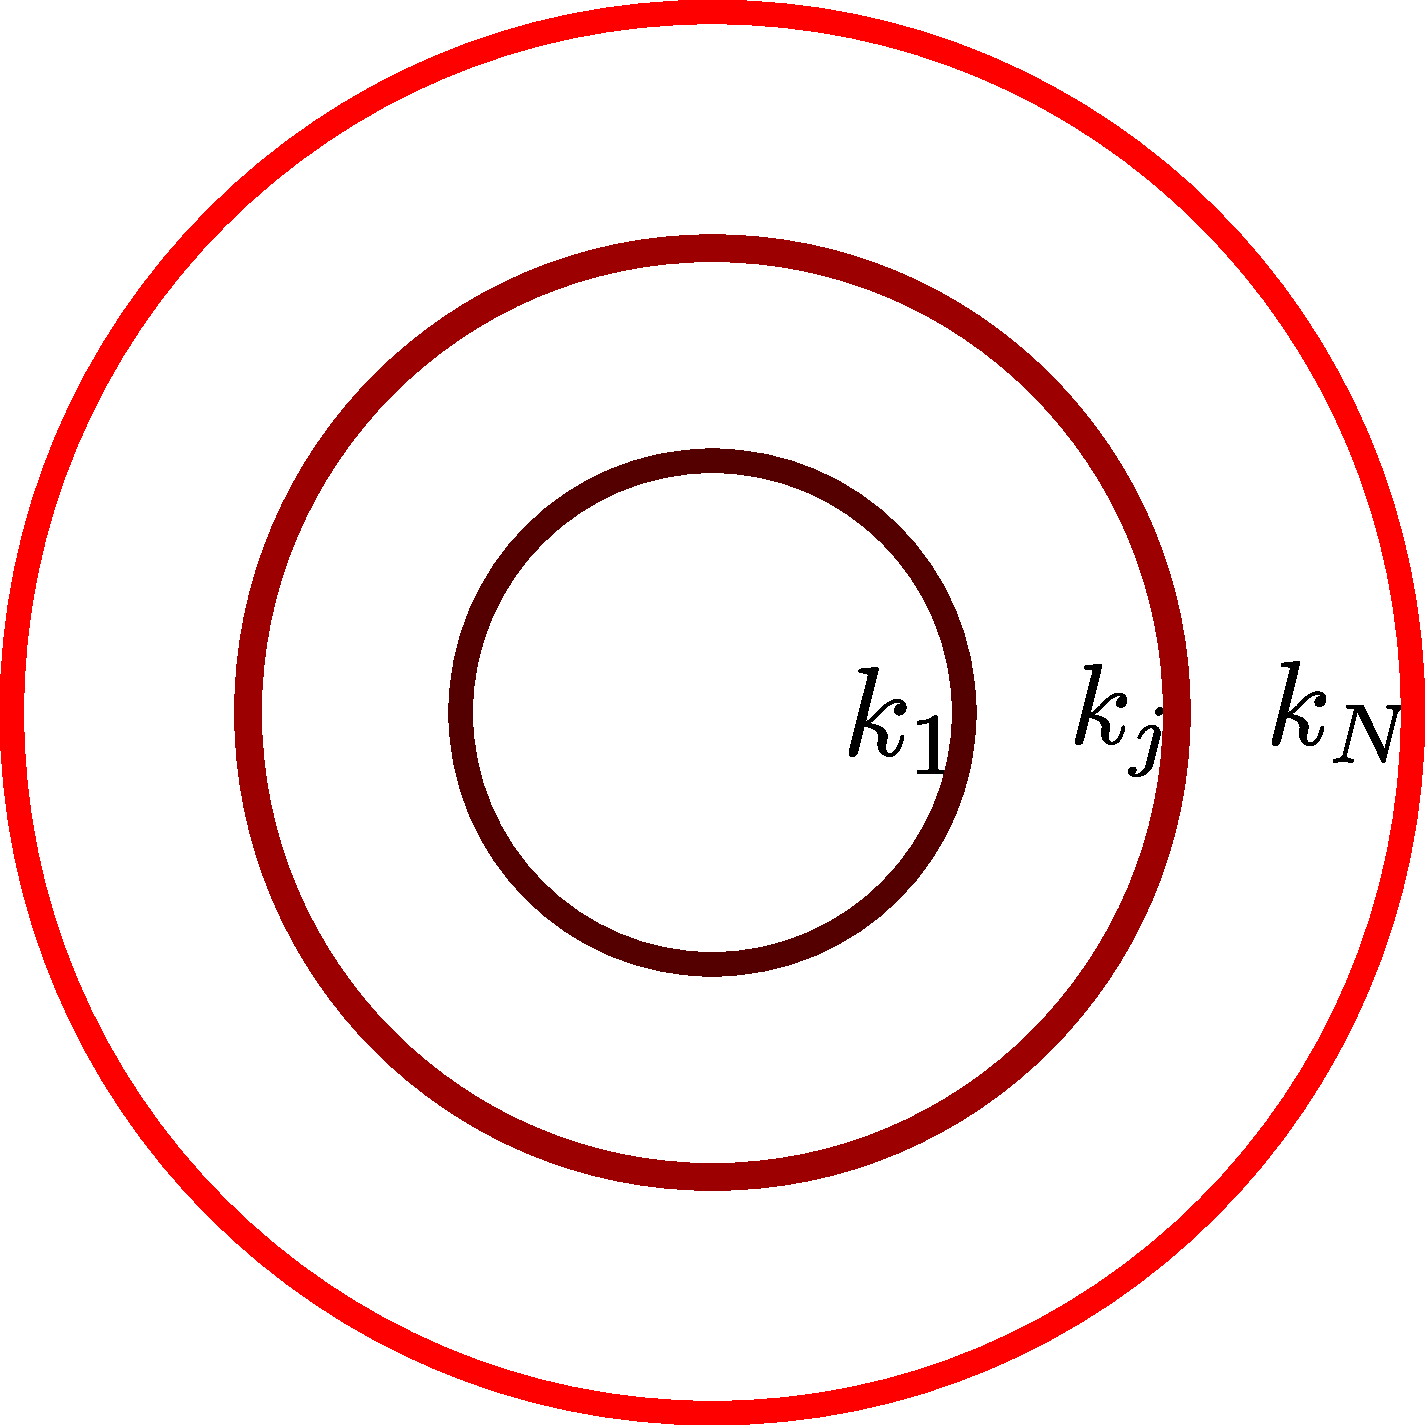
\includegraphics[width=0.9\textwidth]{figures/uv_ir_scheme.pdf}
\end{minipage}
\vspace*{\fill}
\end{frame}

\begin{frame}[noframenumbering]{The Unitary RG Method: Write Hamiltonian in the basis of \(\vec k_j\)}
\vspace*{-20pt}
\vspace*{\fill}

\begin{minipage}{0.4\textwidth}
	\vspace*{-30pt}
	\[H_{(j)} = H_1 \hat n_j + H_0 \left(1 - \hat n_j\right) + c^\dagger_j T + T^\dagger c_j\]
\[
 {2^{j-1} \text{-dim.}} \longrightarrow \begin{cases}
	H_1, H_0 \longrightarrow \text{diagonal parts}\\
T \longrightarrow \text{off-diagonal part}
\end{cases}
\]
\[ (j) : j^\text{th} \text{ RG step}\]
\end{minipage}
\hspace*{\fill}
\begin{minipage}{0.5\textwidth}
\begin{figure}
	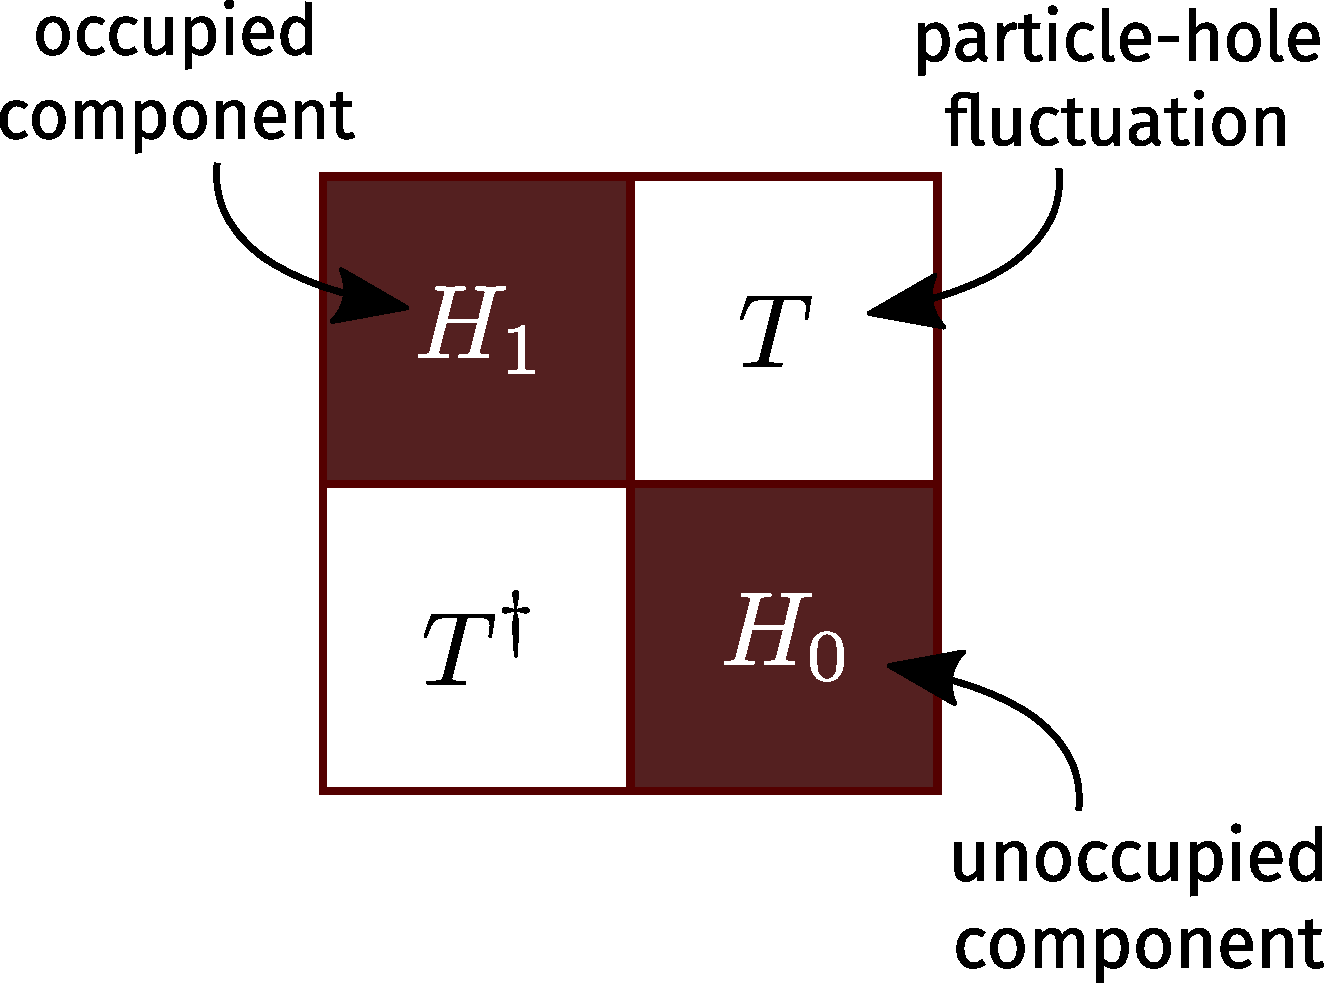
\includegraphics[width=0.9\textwidth]{figures/urg_ham.pdf}
\end{figure}
\end{minipage}
\end{frame}

\begin{frame}[noframenumbering]{The Unitary RG Method: Rotate Hamiltonian and kill off-diagonal blocks}

\vspace*{\fill}

\begin{minipage}{0.45\textwidth}
\centering
\[H_{(j-1)} = U_{(j)} H_{(j)} U_{(j)}^\dagger\]
\[U_{(j)} = \frac{1}{\sqrt 2}\left(1 - \eta_{(j)} + \eta_{(j)}^\dagger\right), ~ ~ \left\{\eta_{(j)}, \eta^\dagger_{(j)}\right\} = 1 \]
\[ \eta^\dagger_{(j)} = \frac{1}{\hat \omega_{(j)} - H_D}c^\dagger_j T \Bigg \} \rightarrow {\text{many-particle}\atop{\text{rotation}}}\]
\[\hat \omega_{(j)} = \left(H_{1} + H_{0}\right)_{(j-1)} + \Delta T_{(j)}\]
\[\hat \omega: \text{\focus{quantum fluctuation} operator}\]
\vspace*{\fill}
\end{minipage}
\hspace*{\fill}
\begin{minipage}{0.5\textwidth}
\begin{figure}
	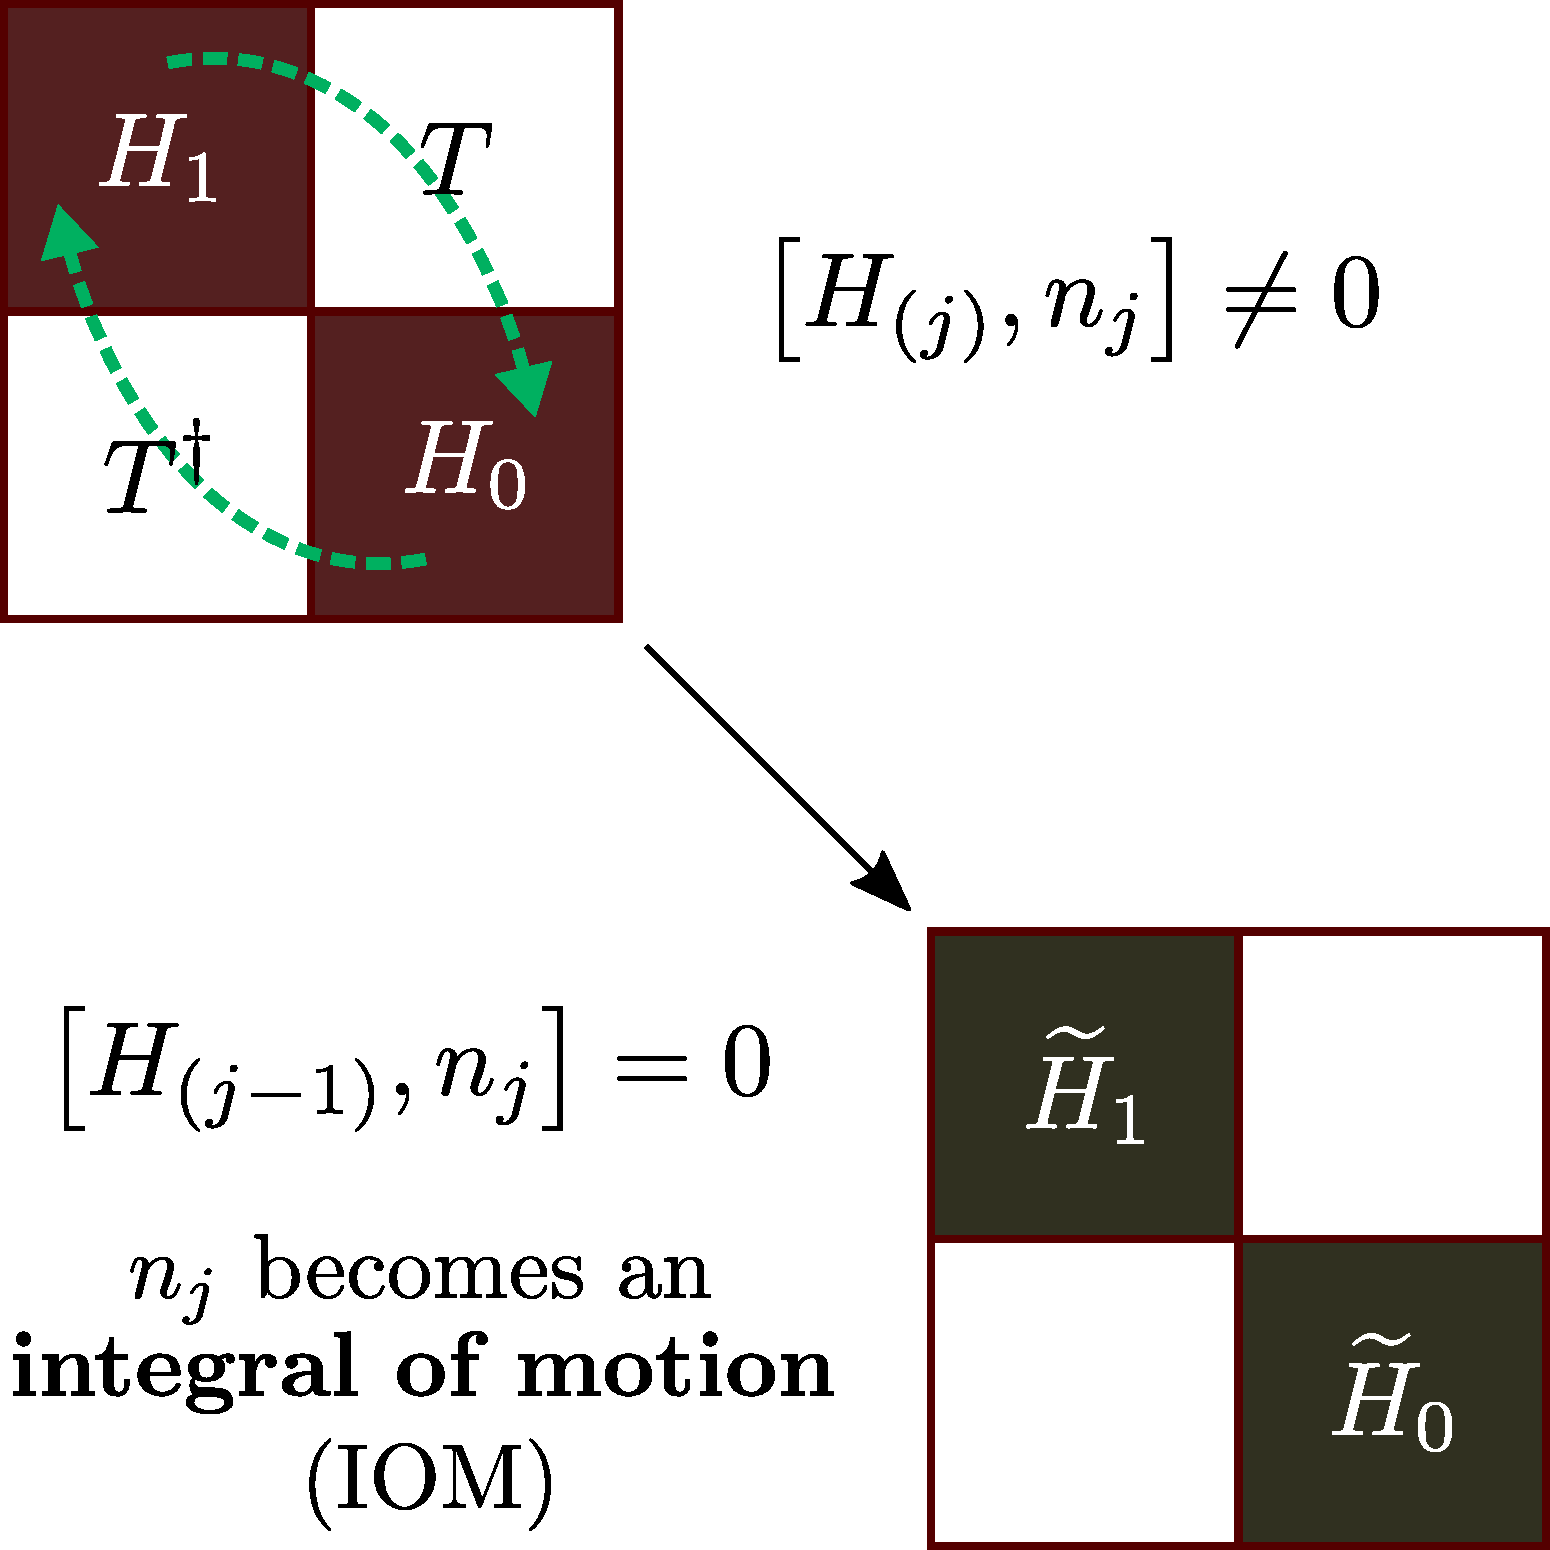
\includegraphics[width=0.8\textwidth]{figures/urg_rot.pdf}
\end{figure}
\end{minipage}
\end{frame}

\begin{frame}[noframenumbering]{The Unitary RG Method: Repeat with renormalised Hamiltonian}

\begin{minipage}{0.53\textwidth}
	\[H_{(j-1)} = \widetilde H_1 \hat n_j + \widetilde H_0 \left(1 - \hat n_j\right)\]
	\[\widetilde H_1 = H_1 \hat n_{j-1} + H_0 \left(1 - \hat n_{j-1}\right) + c^\dagger_{j-1} T + T^\dagger c_{j-1}\]
\vspace*{\fill}
\end{minipage}
\hspace*{\fill}
\begin{minipage}{0.45\textwidth}
\begin{figure}
	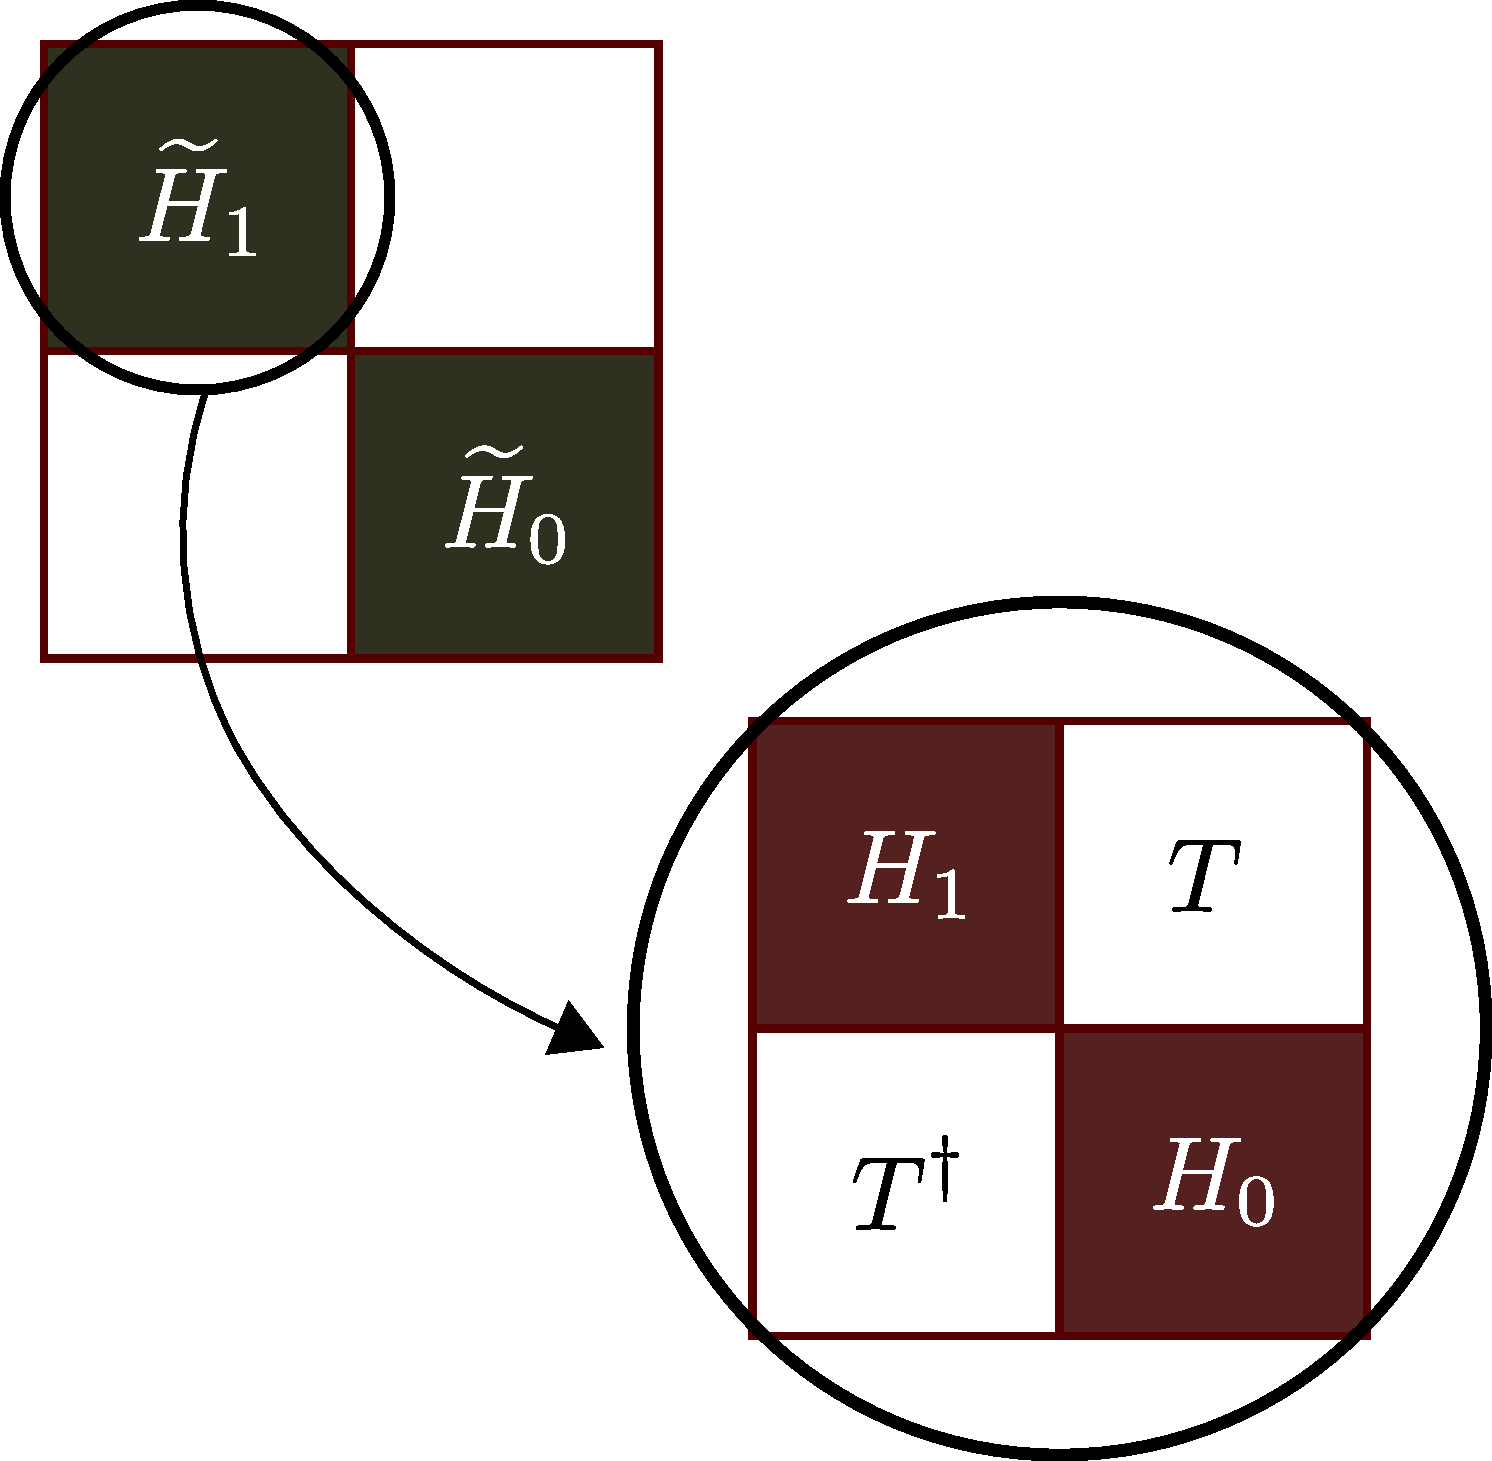
\includegraphics[width=\textwidth]{figures/urg_next.pdf}
\end{figure}
\end{minipage}
\end{frame}

\begin{frame}[noframenumbering]{The Unitary RG Method: RG Equations and Denominator Fixed Point}

\begin{minipage}{0.55\textwidth}
	\centering
\[ \Delta H_{(j)} = \left(\hat n_j - \frac{1}{2}\right) \left\{c^\dagger_j T, \eta_{(j)}\right\} \]
\[\eta^\dagger_{(j)} = \frac{1}{\hat \omega_{(j)} - H_D}c^\dagger_j T\] 
\[\text{{Fixed point:}}~ ~ ~\hat \omega_{(j^*)} - \left(H_D\right)^* = 0\]
\focus{eigenvalue of \(\hat \omega\) coincides with that of \(H\)}
\end{minipage}
\hspace*{\fill}
\begin{minipage}{0.4\textwidth}
	\centering
	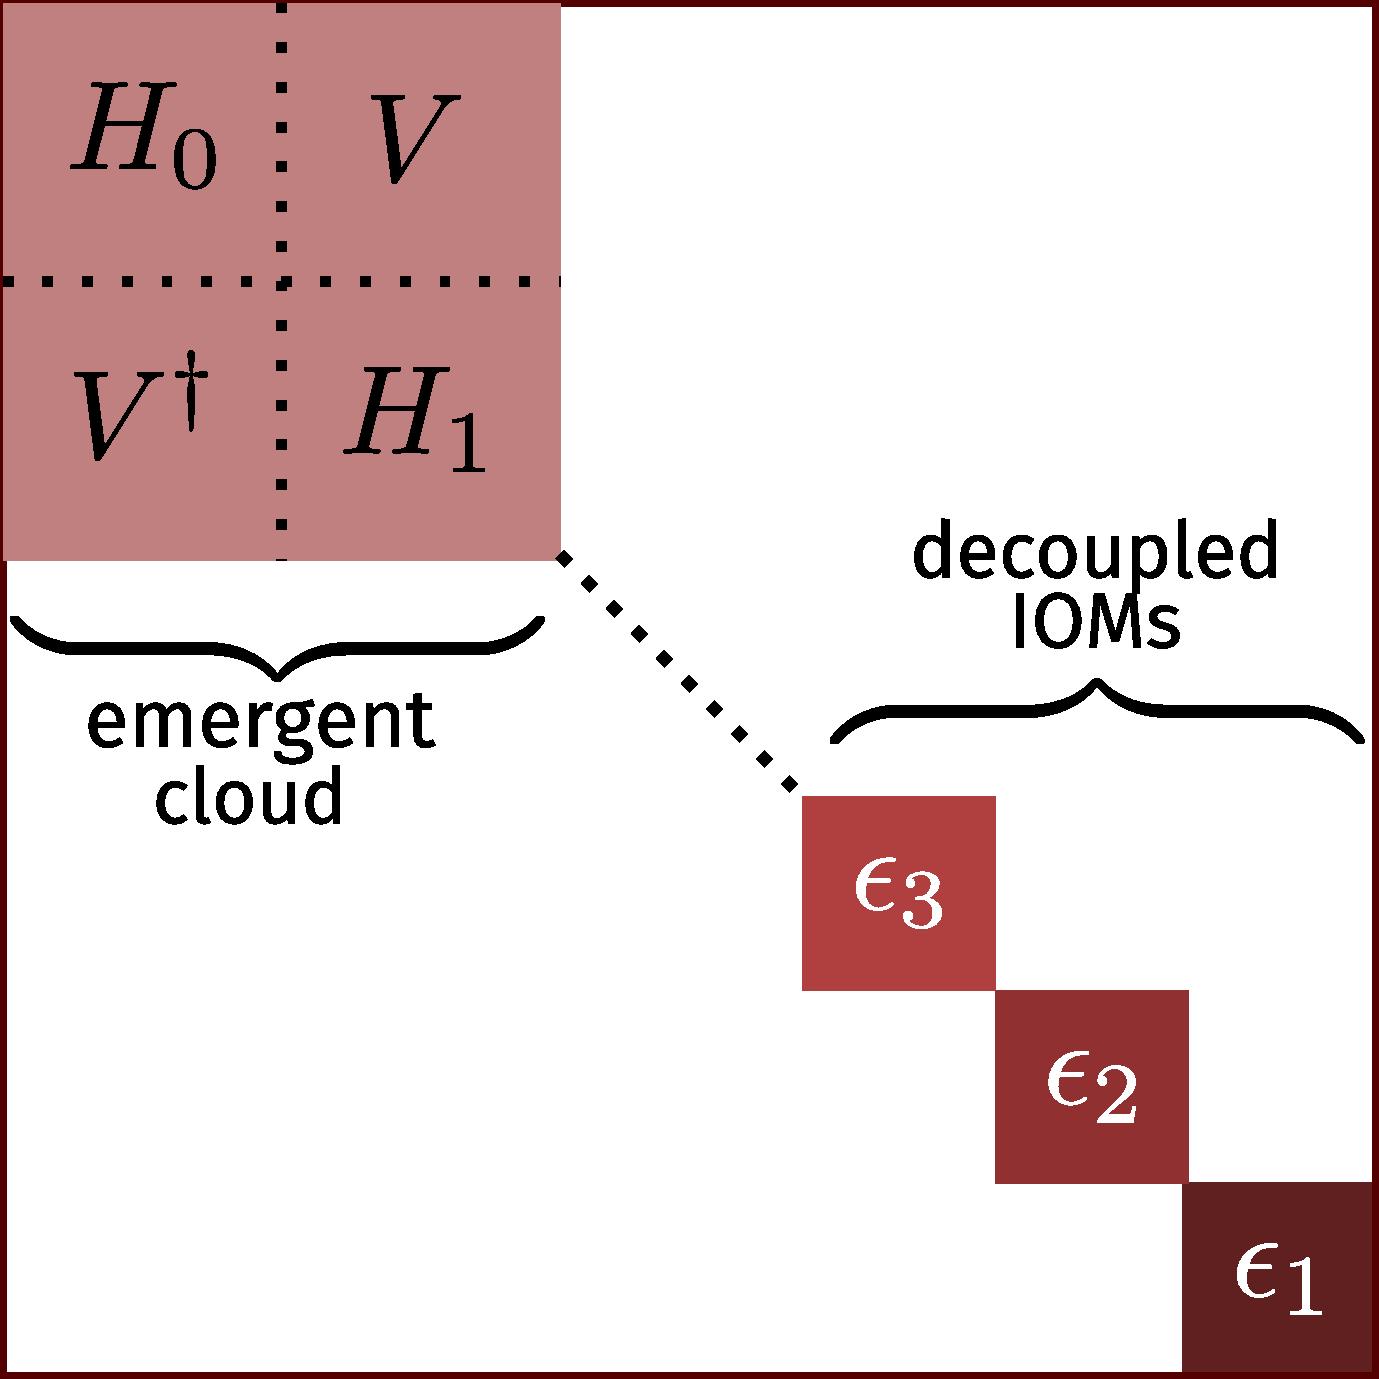
\includegraphics[width=0.9\textwidth]{figures/urg_ham_full.pdf}
\end{minipage}
\vspace*{\fill}
\end{frame}

\begin{frame}[noframenumbering]{The Unitary RG Method: Novel Features of the Method}

\begin{minipage}{0.65\textwidth}
\begin{itemize}[<+->]
	\item \focus{Quantum fluctuation scale} \(\hat \omega\)	that tracks all orders of renormalisation\\[10pt]
	\item Finite-valued fixed points for finite systems - leads to \focus{emergent degrees of freedom}\\[10pt]
	\item \focus{Spectrum-preserving} unitary transformations - partition function does not change\\[10pt]
	\item Tractable low-energy effective Hamiltonians - allows \focus{renormalised perturbation theory} around them 
\end{itemize}
\end{minipage}
\hspace*{\fill}
\begin{minipage}{0.3\textwidth}
\centering
\(H_{(j-1)} = U_{(j)} H_{(j)} U_{(j)}^\dagger\)\\[15pt]
\(U_{(j)} = \frac{1}{\sqrt 2}\left(1 - \eta_{(j)} + \eta_{(j)}^\dagger\right) \)\\[15pt]
\( \eta^\dagger_{(j)} = \frac{1}{\hat \omega_{(j)} - H_D}c^\dagger_j T\)\\[15pt]
\( \Delta H_{(j)} = \left(\hat n_j - \frac{1}{2}\right) \left\{c^\dagger_j T, \eta_{(j)}\right\} \)
\end{minipage}
\end{frame}

\section{Final Remarks}
\label{concl}

\begin{frame}[noframenumbering]{Conclusions}
	\begin{itemize}[<+->]
		\item The auxiliary model method described here provides a \focus{constructionist} approach to studying systems of strong correlations
		\item \focus{Minimal attractive interaction} on bath leads to a metal-insulator transition in the Hubbard-Heisenberg model
		\item The transition derives from a competition between \focus{Kondo} spin-flip physics and the physics of \focus{pairing} instability.
\end{itemize}
\end{frame}

\begin{frame}[noframenumbering]{Moving forward}
\begin{itemize}[<+->]
	\item \(\vec k-\)dependence of the self-energy: \focus{electronic differentiation} and effects of Van Hove singularities?
	\item Breaking particle-hole symmetry on the impurity will allow us to study bulk models \focus{away from half-filling}.
	\item For more accurate results, one can consider \focus{multiple impurities} in the cluster.
\end{itemize}
\end{frame}

\section{Thank you.}


\end{document}
